\chapter{Conclusion}

We started with a remind of the quantale-valued relations
and the quiet observation that composing them is already a form of optimization,
transitivity being its simplest instance. From there, we recalled and refined the graphical theory
of polyhedral relations, giving it a home inside this same categorical
hierarchy rather than treating it as a self-contained formalism. On that
foundation, we built \textbf{GLP}, a graphical algebra for parametric linear
programs: a single new generator for the linear objective, a handful of
axioms, and a proof that these suffice, both for completeness and for a
normal form (Theorem~\ref{thm:NormalFormGLP}).

Three results are worth calling out on their own. First, \textbf{GLP} is
\emph{complete}: any two diagrams with the same semantics can be rewritten
into one another using only the axioms of the algebra, so there is no gap
between what the theory can prove equal and what is actually equal. Second,
every such diagram admits a \emph{normal form}
(Theorem~\ref{thm:NormalFormGLP}), a canonical shape that every parametric
linear program reduces to, which is what makes the correspondence with value
functions below more than a loose analogy. Third, one of the axioms encodes
something genuinely structural about linear programming rather than
something we imposed on it: the \emph{invariance of a linear program under
column-stochastic reweighting of its objective} (Remark~\ref{rmk:stochastic})
falls directly out of the algebra, as a single generator-level equation,
instead of being proved separately for each formulation. This is one of the 
core properties of linear systems and thanks to our Graphical Algebra is 
a syntatical operation in itself. As we claimend at the introduction,
the diagrammatic calculi makes the system properties evident in the syntax, 
instead of a higher level result and this is the evidence.

A linear program is now a morphism like any other in the hierarchy, one that composes with the
relations and quadratic blocks studied earlier without any special
pleading. Its diagrammatic syntax, once reduced to normal form, coincides
with the syntax of its own value function, so the diagram and the object it
computes are, in a precise sense, the same picture drawn twice.

Just like that, other theories can be developed by enriching the here presented
language. Figure~\ref{fig:overview} lays out the resulting hierarchy of categorical
structures that were developed by this very recipe and what can actually be achieved
in the end of the road.

\begin{figure}[H]
	\centering
	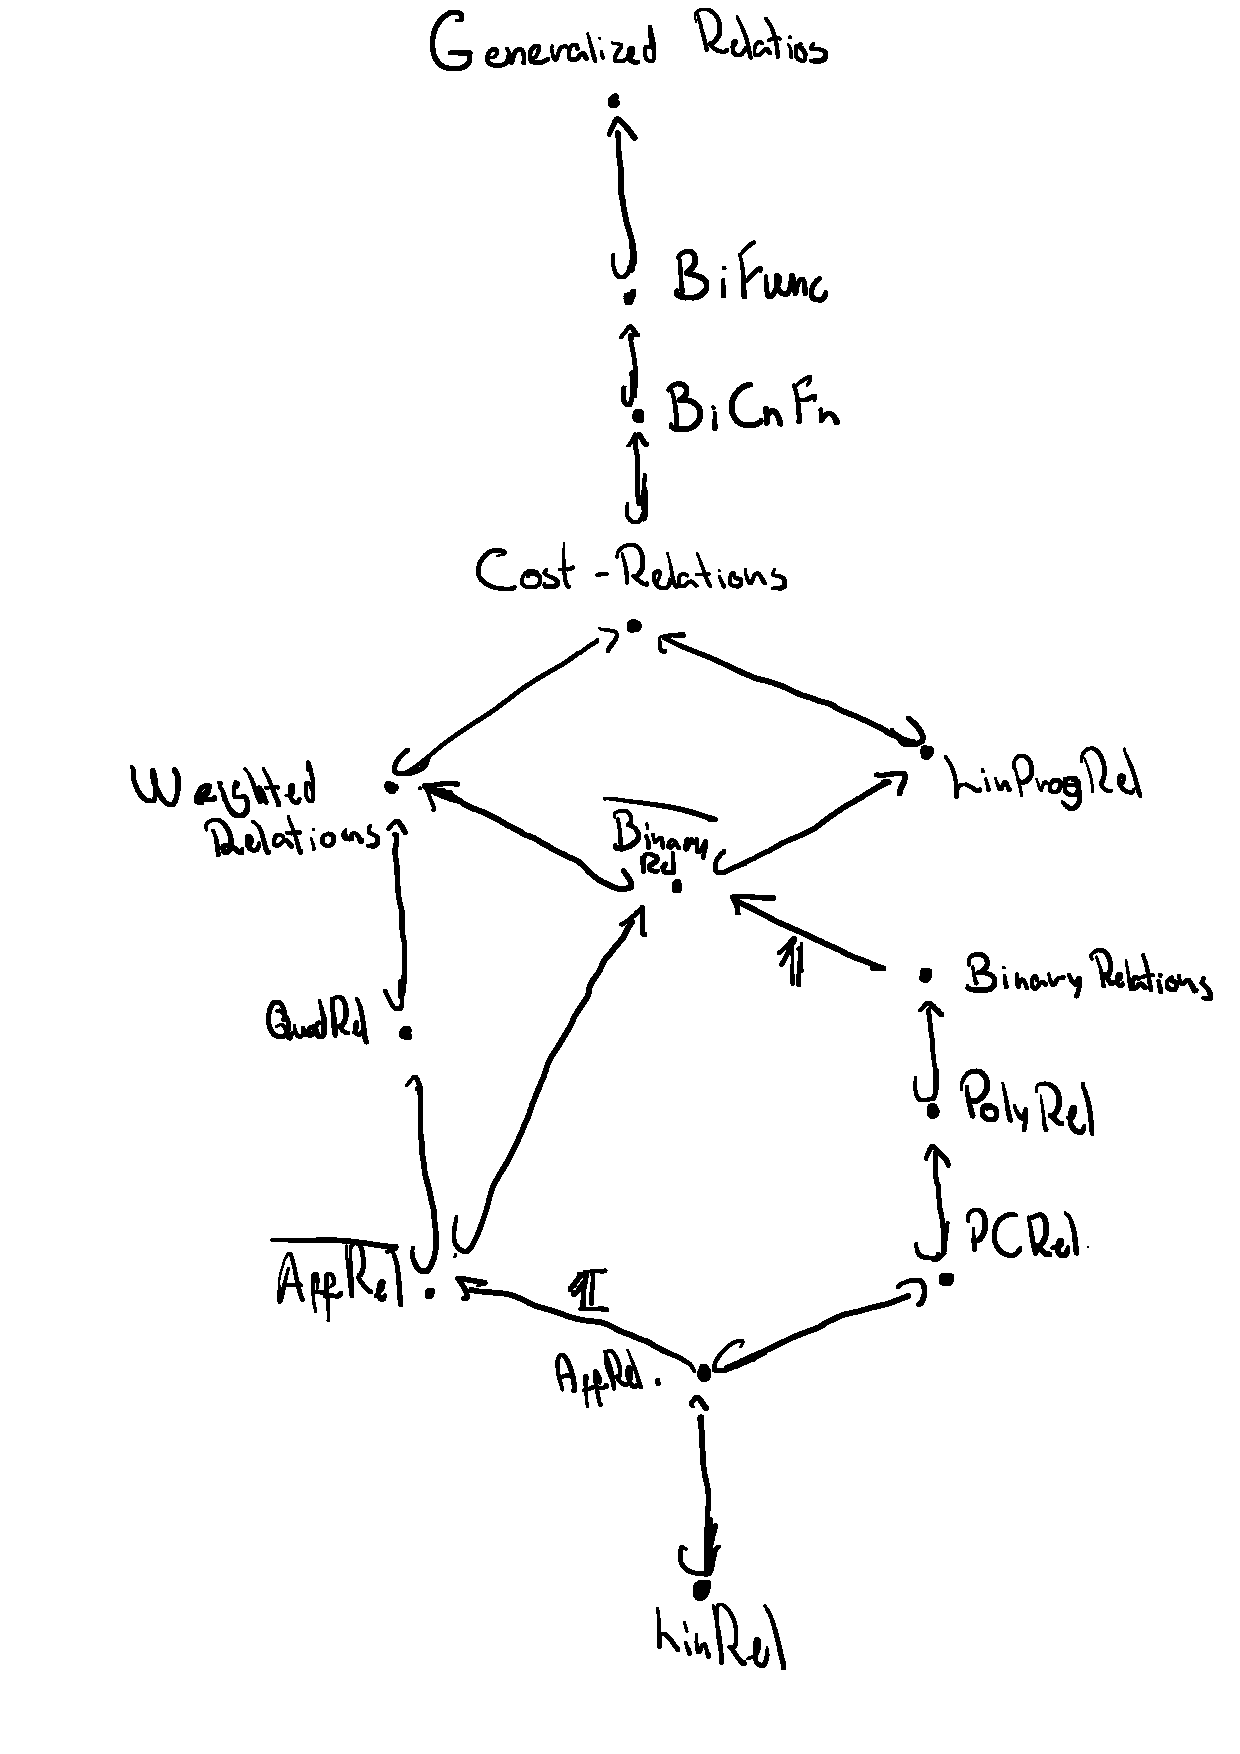
\includegraphics[width=1.0\linewidth]{images/Overview.pdf}
	\caption{The hierarchy of relational categories developed in this
		thesis. Each inclusion preserves the monoidal and compositional
		structure of the layer below.}
	\label{fig:overview}
\end{figure}

\begin{itemize}
	\item Moving upward corresponds to increasing expressive power: each
	      layer generalises the one below by enlarging the class of morphisms,
	      while preserving the compositional structure.
	\item The morphisms marked $\hookrightarrow$ are inclusion functors,
	      embedding each category as a full subcategory of the one above.
	\item The morphism marked $\mathbf{1}$ denotes the indicator function
	      embedding, which sends a set-valued relation to its
	      $\{0,+\infty\}$-valued characteristic function.
\end{itemize}

It is a modest step, in the end, toward something larger: a diagrammatic 
and more calculational language expressive enough to hold optimization in its own right.
The theories presented and developed here
read less like separate constructions sharing a notation and one theory
examined at different levels of resolution. A sequential increment of the theory,
one generator at a time, lifting the whole theory.
